\documentclass[11pt]{article}
\usepackage[margin=1in]{geometry}
\usepackage{amsmath,amssymb,booktabs,graphicx,hyperref,longtable,caption,microtype,float}
\usepackage[section]{placeins}
\hypersetup{colorlinks=true,linkcolor=blue,urlcolor=blue,citecolor=blue}
\graphicspath{{../../img/compass/}{../../outputs/compass/}}
\newcommand{\R}{\mathbb{R}}
\newcommand{\E}{\mathbb{E}}
\title{A Hidden Political Compass from Aggregate Election Returns,\\ and What It Implies for Alternative Voting Methods}
\author{Brian Bell}
\date{November 15, 2026 \\[2pt] \small Working draft. All numbers are produced by the code in \texttt{compass/} and \texttt{scripts/}.}

\begin{document}
\maketitle

\begin{abstract}
We fit a low-dimensional latent ``political compass'' to U.S.\ presidential, Senate and House returns for 1976--2020 (10{,}528 contested races) using only aggregate vote shares. Each state is a slowly drifting mixture of a few fixed national voter types; candidates live in the same space; voters choose probabilistically by distance. On held-out races the model matches or beats a strong non-spatial regression baseline for House and presidential state results and ties it for Senate. Only the Democrat--Republican axis is stably identified; the second axis is not. We then draw simulated voters from the fitted compass, calibrated so their first choices reproduce every real result, and re-run all 10{,}774 House and Senate contests under ranked choice, approval, STAR, Borda, Condorcet and random-ballot rules. With sincere voters and the observed candidate field, the deterministic rules almost never change the winner. We measure the suppression of third-party support in two ways: a closeness gradient (small, $0$--$0.5$) and a comparison with contests in which only one major party ran (large, $0.64$--$0.89$ by year). Under the larger estimate, third parties win 4--5 House seats per election under every rule, and about 34 under random ballot. In all scenarios, whether voters are sincere matters more than which deterministic rule counts the ballots.
\end{abstract}

\tableofcontents

\section{Data}
\label{sec:data}
Source files are the 1976--2020 constituency returns in \texttt{csv/} for president (by state), Senate and House, and two Gallup party-identification series (2004--2024).

\paragraph{Race table for fitting.} General elections only. Fusion-ticket lines are summed per candidate. Write-in totals, blank and scattering rows are dropped. Candidates below $5\%$ of the named-candidate vote are dropped and the remaining shares renormalised; races with fewer than two remaining candidates are dropped. This leaves $10{,}528$ races: $611$ presidential state-years, $775$ Senate, $9{,}142$ House.

\paragraph{Incumbency.} Derived, not given: a candidate is an incumbent if the same person (matched on surname and first initial within a state) won that office two years earlier (House) or within six years (Senate).

\paragraph{Contest table for simulation.} All House and Senate general-election contests, keeping every candidate above $0.5\%$ (at most six) and keeping uncontested seats as automatic wins: $10{,}774$ contests, of which $4{,}783$ have three or more candidates. Party groups are Democrat, Republican, Libertarian, Green and other.

\paragraph{Party identification.} Gallup's party series (Republican / independent / Democrat) and leaner series (Republican incl.\ leaners / Democrat incl.\ leaners) combine into five groups: Democrat, lean Democrat, pure independent, lean Republican, Republican. The 2004--2020 means are $31.7 / 15.8 / 10.1 / 13.8 / 28.5\%$.

\section{The compass model}
\label{sec:model}

\FloatBarrier
\subsection{Voters}
There are $K$ national voter types. Type $k$ is a Gaussian cloud in $\R^d$,
\begin{equation}
z \mid k \sim \mathcal N\!\left(\mu_k, \operatorname{diag}(\sigma_k^2)\right), \qquad k=1,\dots,K ,
\end{equation}
fixed over time. State $s$ in year $t$ is a mixture of the types with weights
\begin{equation}
\pi_{s,t} = \operatorname{softmax}\!\left(A_s + B_s\,\tau_t\right), \qquad \tau_t = (t-1998)/22 ,
\end{equation}
and a House district $u$ (keyed by redistricting era) adds an offset $G_u$ to its state's logits. Defaults are $d=2$, $K=4$. Fixing the types over time is the assumption that anchors the space: populations drift slowly, candidates and parties move.

\FloatBarrier
\subsection{Candidates}
Candidate $j$ has a position $c_j\in\R^d$ and a scalar valence $v_j$.
\begin{align}
c_j &= p_{P(j),t} + \lambda\,(m_{u,t}-\bar m_t) && \text{major-party House/Senate} \\
c_j &= p_{P(j),t} + \delta_j && \text{presidential} \\
c_j &= \delta_j && \text{third-party / independent}
\end{align}
Here $p_{P,t}$ is party $P$'s position in year $t$, following a Gaussian random walk with step s.d.\ $0.03$; $m_{u,t}=\pi_{u,t}^{\top}\mu$ is the constituency mean, $\bar m_t$ the national mean, and $\lambda\in(0,1)$ a learned adaptation rate. Individual positions are estimated only where identifiable (a presidential candidate faces 51 electorates; a congressional candidate usually one). Valence is
\begin{equation}
v_j = \big(w_{0,o} + w_{t,o}\big)\,\mathbf 1[j \text{ Democrat}] + \beta_o\,\mathrm{inc}_j + u_j ,
\end{equation}
with $w_{0,o}$ the long-run Democratic advantage for office $o$, $w_{t,o}$ that year's national swing (shrunk to zero), $\beta_o$ an incumbency bonus and $u_j$ a per-candidate effect shared across a person's races.

\FloatBarrier
\subsection{Voting and likelihood}
A voter at $z$ chooses candidate $j$ with probability
\begin{equation}
P(j\mid z) = \frac{\exp\!\left(-\lVert z-c_j\rVert^2 + v_j\right)}{\sum_{l}\exp\!\left(-\lVert z-c_l\rVert^2 + v_l\right)} ,
\label{eq:choice}
\end{equation}
the random-utility form of ``vote for the nearest candidate'': $U_{ij} = -\lVert z_i-c_j\rVert^2+v_j+\varepsilon_{ij}$ with $\varepsilon_{ij}$ i.i.d.\ Gumbel. The predicted share in race $r$ is
\begin{equation}
\hat y_{rj} = \sum_k \pi_{r,k}\; \E_{z\sim k}\big[P(j\mid z)\big],
\end{equation}
with the expectation taken over $M=64$--$128$ scrambled-Sobol points per type. Observed shares follow
\begin{equation}
y_r \sim \operatorname{Dirichlet}\!\left(\phi_{o(r)}\,\hat y_r\right), \qquad \phi = (1000, 300, 300) \text{ for president, Senate, House.}
\end{equation}
$\phi$ is fixed, not learned: with one race per congressional candidate, a learned $\phi$ diverges as the $u_j$ absorb each race.

\FloatBarrier
\subsection{Priors and fitting}
All priors are zero-mean Gaussians: $\mu_k$ (s.d.\ $1.5$), $A_s$ ($2$), $B_s$ ($1$), $G_u$ ($1$), party random-walk steps ($0.03$), presidential $\delta_j$ ($0.5$), other $\delta_j$ ($1$), presidential $u_j$ ($1$), congressional $u_j$ ($0.5$), $w_{t,o}$ ($0.5$). The fit is maximum a posteriori by full-batch Adam with cosine learning-rate decay ($1{,}200$ steps, about three minutes on a laptop CPU). The result is a point estimate, not a posterior over parameters.

\FloatBarrier
\subsection{Identification}
The space has no intrinsic orientation; for display, axis~1 is the mean Democrat-to-Republican direction. A uniform national shift in voters is observationally equivalent to a national swing in one year, so slow movement is assigned to positions and mixtures and fast movement to $w_{t,o}$. Two specification choices (the tight party random walk and linear rather than quadratic state trends) were made after the first forward forecast failed, so the forward test below is slightly optimistic.

\section{Does the model reproduce real elections?}
\label{sec:validation}

\paragraph{Baseline.} Ridge regression on the logit of the two-party Democratic share with state effects, per-state linear trends, year$\times$office effects, incumbency by office and House-district effects.

\paragraph{Metric.} Root-mean-square error of the Democratic share of the two-party vote, in percentage points, on races not used in fitting.

\begin{table}[H]\centering
\caption{Held-out error (percentage points). Random split: three independent $20\%$ hold-outs. Forward split: fit on 1976--2016, predict 2018--2020 with no information from those years.}
\begin{tabular}{llrrr}
\toprule
Test & Office & $n$ & Compass & Baseline \\
\midrule
Random $20\%$ & President (state) & $\approx122$ & \textbf{3.6} (3.3 / 3.6 / 4.1) & 4.6 \\
 & Senate & $\approx150$ & 7.9 (8.2 / 7.8 / 7.6) & 7.8 \\
 & House & $\approx1{,}700$ & \textbf{6.7} (6.6 / 6.7 / 7.0) & 7.8 \\
\midrule
Forward & President 2020 & 51 & 5.7 & \textbf{4.0} \\
 & Senate & 64 & \textbf{5.6} & 7.9 \\
 & House & 794 & \textbf{7.3} & 7.7 \\
\bottomrule
\end{tabular}
\end{table}

\paragraph{Calibration.} A Beta concentration per office is fitted on half of the held-out races and coverage of the central $90\%$ interval is checked on the other half. Random splits: president $0.91$--$0.94$, Senate $0.84$--$0.88$, House $0.90$--$0.92$, with mean half-widths of about $6$, $13$ and $11$ points.

\paragraph{Dimension.} On one random split, $(d,K)=(1,3)$ gives $3.6/8.5/6.6$ for president/Senate/House, $(2,4)$ gives $3.3/8.2/6.6$, and $(3,6)$ gives $4.5/8.1/6.7$. One dimension carries nearly all of the predictive value.

\paragraph{Identifiability.} Across three random restarts on the real data, state-year positions on the party axis correlate at $0.88$, but the full two-dimensional maps agree only at Procrustes $R^2 = 0.64$--$0.69$. Refitting simulated elections drawn from a known compass on the real race design recovers the party axis at $0.94$ and the full map at $R^2=0.65$, with held-out error of $4.2$--$5.2$ points against a noise floor of $2.6$--$2.8$. The second axis should not be interpreted.

\paragraph{Face validity.} The most Democratic states on axis~1 are DC, GA, WV, AR, TN, MD in 1976 and DC, MA, CA, HI, NY, IL in 2020; the party positions move apart over the period; fitted House swings have the expected sign in 2006, 2008, 2010, 2014 and 2018. The adaptation rate is $\lambda\approx0.04$.

\begin{figure}[!htbp]\centering
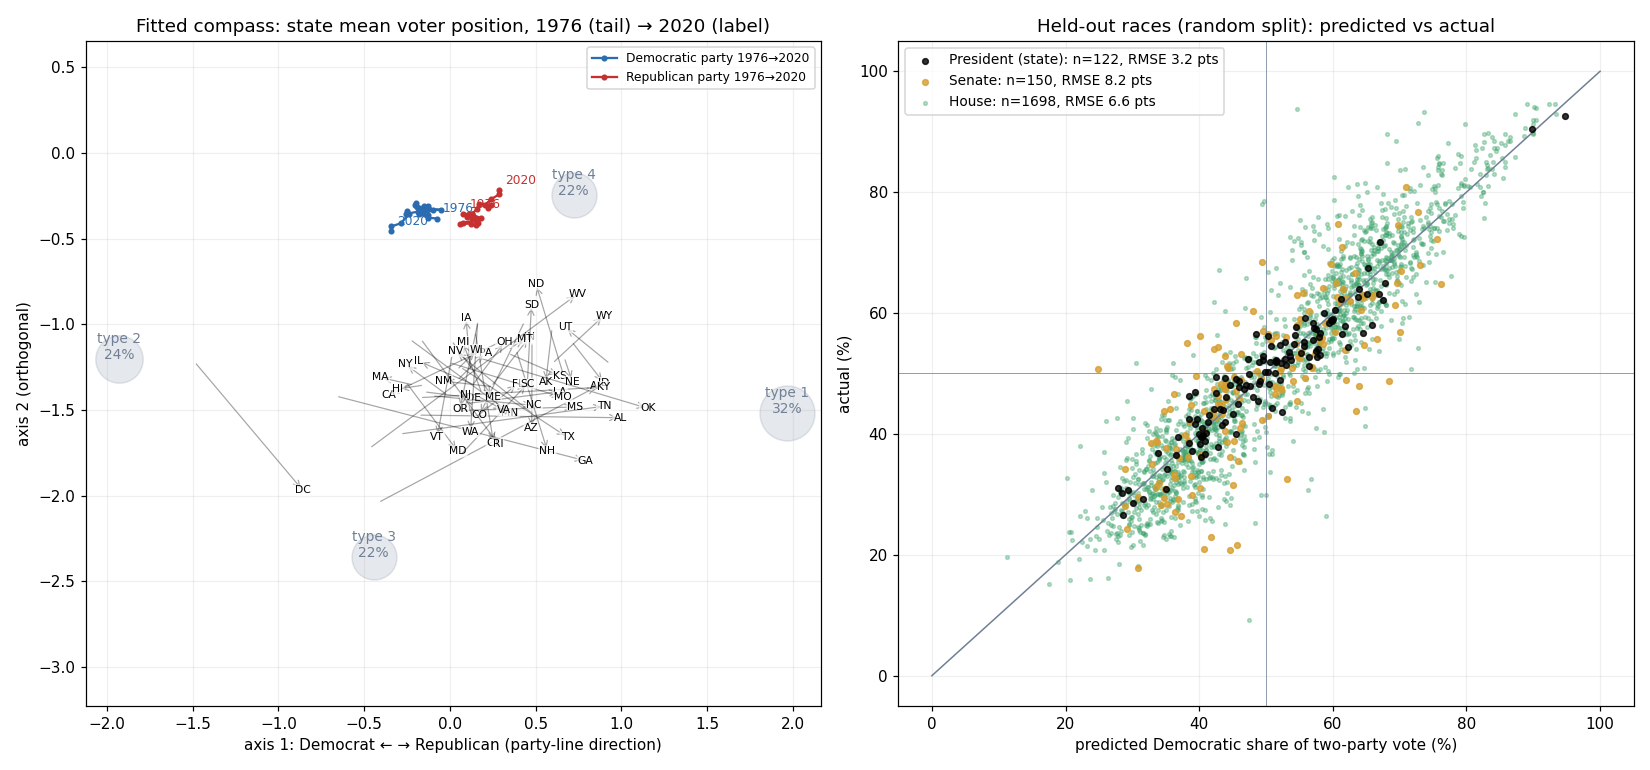
\includegraphics[width=\textwidth]{PSH_random_d2K4_s0.png}
\caption{Left: fitted state mean positions, 1976 (arrow tail) to 2020 (label), with voter types and party paths. Right: predicted against actual Democratic two-party share on held-out races.}
\end{figure}

\paragraph{Party identification check.} For each agent define the partisan gap $g = U_{D}-U_{R}$ for generic party candidates in the House environment, plus a logistic taste shock. With two thresholds fixed across years, $|g|<0.3$ (pure independent), $0.3$--$1.2$ (leaner), $>1.2$ (identifier), the compass gives $32.5/14.4/10.2/14.9/27.9\%$ against Gallup's $31.7/15.8/10.1/13.8/28.5\%$ (year-by-group RMSE $3.7$ points). The compass's yearly net Democratic lean correlates with Gallup's at $0.87$ over nine election years. Gallup was not used in fitting.

\section{Simulating other voting methods}
\label{sec:methods}

\FloatBarrier
\subsection{Calibration to real first choices}
Minor-party candidates not covered by the main fit receive one position per group (Libertarian, Green, other), estimated by maximising the multinomial likelihood of all shares with major-party candidates held fixed. Then, for each contest, valences are solved by the fixed-point iteration
\begin{equation}
v_j \leftarrow v_j + \log y_j - \log \hat y_j(v)
\end{equation}
until expected first-choice shares equal the real shares. The largest absolute error over all contests is $10^{-5}$.

\FloatBarrier
\subsection{Agents and ballots}
Each run draws $N=1{,}000$ agents per contest: a type $k\sim\pi$, a position $z\sim\mathcal N(\mu_k,\sigma_k^2)$, and utilities $U_{ij}=-\lVert z_i-c_j\rVert^2+v_j+\varepsilon_{ij}$. By construction the agents' first choices reproduce the real result in expectation. Two-candidate contests are resolved by a binomial draw, since all majoritarian rules agree there. Ballots are sincere functions of $U$:
\begin{itemize}\itemsep1pt
\item \textbf{Plurality}: most first choices (control).
\item \textbf{Random ballot}: the first choice of one randomly drawn voter (the original ``dice roll'').
\item \textbf{Ranked choice}: instant runoff on the full ranking.
\item \textbf{Approval}: approve $j$ if $U_{ij}\ge\sum_l q_l U_{il}$ with $q$ the poll shares (``better than what I expect to get''). The unweighted mean is also examined.
\item \textbf{STAR}: scores $\operatorname{round}\!\big(5\,(U_{ij}-\min_l U_{il})/(\max_l U_{il}-\min_l U_{il})\big)$; top two by total, then a head-to-head runoff.
\item \textbf{Borda}: one point for each candidate ranked below.
\item \textbf{Condorcet}: the head-to-head winner; minimax margin if there is a cycle.
\end{itemize}
Seats are counted as in the original scripts: House seats won that year; for the Senate, the sitting chamber (most recent contest for each state's seat within three cycles). Each configuration is run 200 times.

\FloatBarrier
\subsection{Baseline result}
\begin{table}[H]\centering
\caption{Mean change in seats relative to the real result, averaged over 23 elections, sincere voters.}
\begin{tabular}{lrrrr}
\toprule
 & \multicolumn{2}{c}{House} & \multicolumn{2}{c}{Senate chamber} \\
Method & Dem. & Rep. & Dem. & Rep. \\
\midrule
Plurality (control) & $-0.1$ & $+0.1$ & $0.0$ & $0.0$ \\
Ranked choice & $-0.1$ & $+0.1$ & $+0.2$ & $-0.2$ \\
Approval & $-0.1$ & $+0.1$ & $+0.2$ & $-0.2$ \\
STAR & $0.0$ & $0.0$ & $+0.3$ & $-0.3$ \\
Condorcet & $-0.1$ & $+0.1$ & $+0.2$ & $-0.2$ \\
Borda & $+0.9$ & $-0.9$ & $+0.9$ & $-0.8$ \\
Random ballot & $-4.8$ & $-4.3$ & $-1.0$ & $-1.0$ \\
\bottomrule
\end{tabular}
\end{table}
Only two contests change winner in more than $90\%$ of runs under ranked choice, STAR and Condorcet: the 1980 New York Senate race (D'Amato $45.1$, Holtzman $43.8$, Javits $11.1$) and California's 1st district in 1990 (Riggs $43.3$, Bosco $41.9$, third candidate $14.8$). Run-to-run standard deviation is about $1.1$ House seats for the deterministic rules and $5.5$ for random ballot. With the unweighted approval threshold, approval shifts about four House seats per election to Democrats, an artefact of fringe candidates lowering the threshold.

\begin{figure}[!htbp]\centering
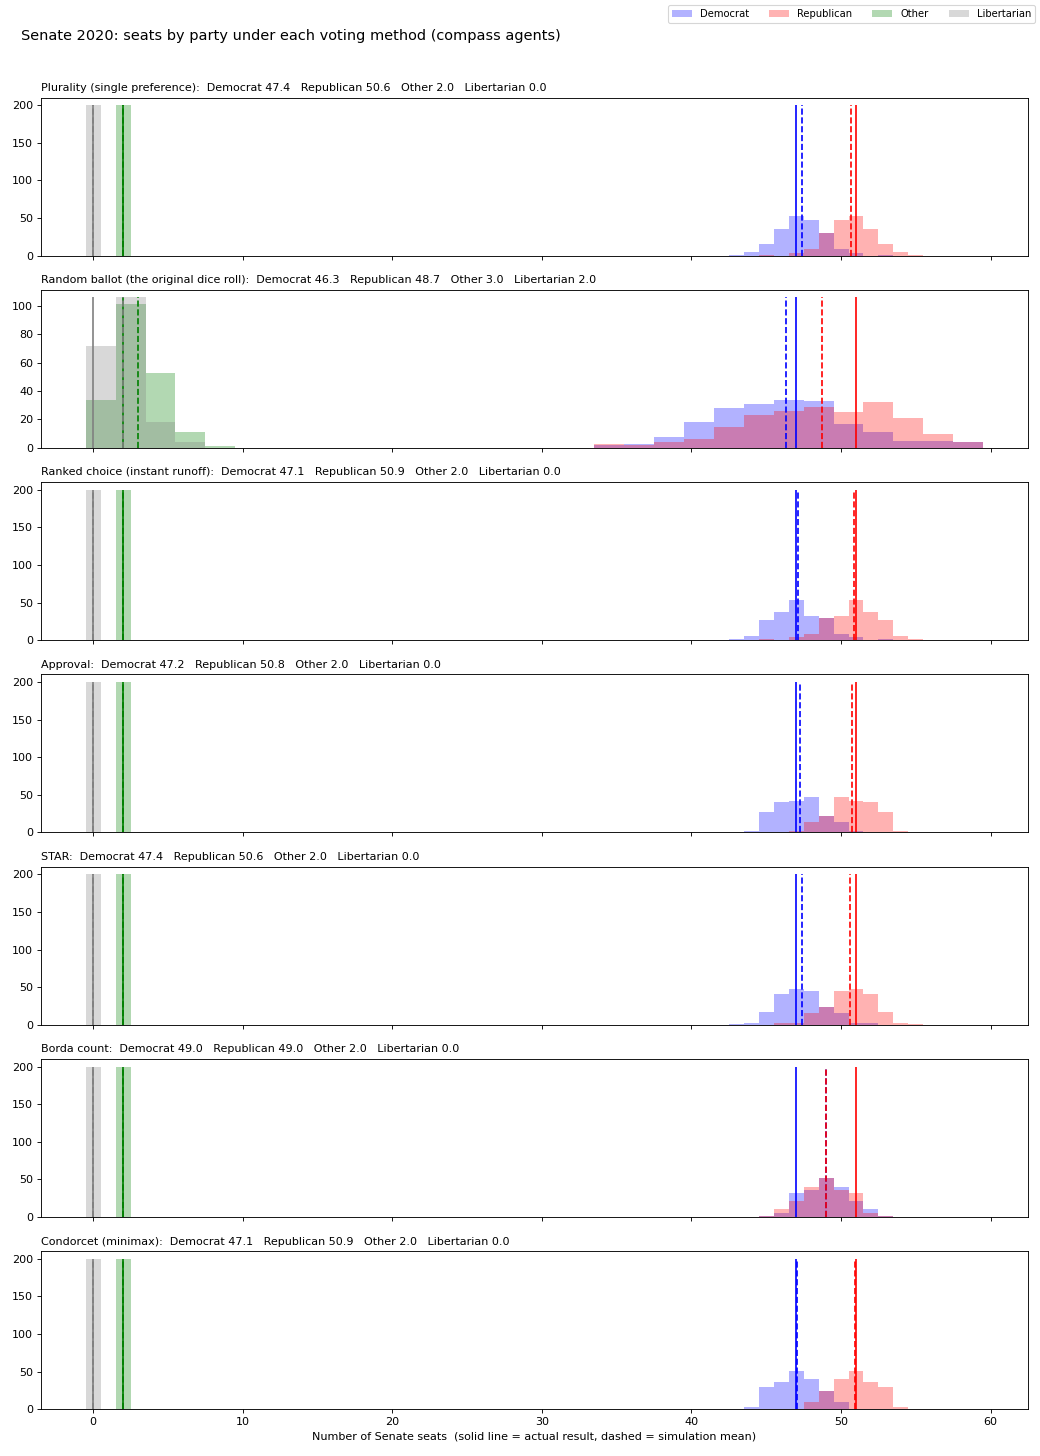
\includegraphics[height=0.82\textheight]{compare/senate-methods-2020.png}
\caption{Senate 2020, sincere baseline: seats by party over 200 runs for each method. Solid lines are the real result, dashed lines the simulation mean.}
\end{figure}

\section{Strategic voting}
\label{sec:strategy}

\FloatBarrier
\subsection{Desertion model}
Let $F_r$ be the two frontrunners of contest $r$. A fraction $\rho$ of voters whose favourite is outside $F_r$ vote instead for the frontrunner they prefer. By the logit second-choice rule the expected strategic-plurality share is
\begin{equation}
s_j(z) =
\begin{cases}
P(j\mid z) + \rho\,\Big(\sum_{m\notin F}P(m\mid z)\Big)\dfrac{P(j\mid z)}{\sum_{f\in F}P(f\mid z)}, & j\in F,\\[8pt]
(1-\rho)\,P(j\mid z), & j\notin F,
\end{cases}
\label{eq:strategic}
\end{equation}
averaged over the electorate. Valences are re-solved so that \eqref{eq:strategic} reproduces the real shares; a third candidate's sincere first-choice share is then approximately its observed share divided by $1-\rho$. $\rho$ is capped per contest so that no third candidate sincerely out-polls the real runner-up.

\FloatBarrier
\subsection{Pragmatic ballots}
Honest ballots follow Section~\ref{sec:methods}. Pragmatic ballots anchor on the frontrunners: plurality and ranked-choice voters place their preferred frontrunner first; approval voters approve everything above the midpoint of the two frontrunners' utilities; STAR voters clamp utilities to the frontrunner interval before scoring, so the preferred frontrunner gets 5 and the other 0.

\FloatBarrier
\subsection{Outcome measures}
\emph{Compass expression} is $-\frac1N\sum_i\lVert z_i-c_w\rVert^2$ for winner $w$. \emph{Condorcet efficiency} is the share of runs electing the honest head-to-head winner. Disproportionality is the Gallagher index against sincere first-choice shares,
\begin{equation}
\mathrm{LSq}=\sqrt{\tfrac12\sum_p\left(\text{seat}\%_p-\text{vote}\%_p\right)^2}.
\end{equation}

\FloatBarrier
\subsection{Measurement 1: the closeness gradient}
If voters abandon third parties when their vote matters, third-party share should fall in close races. Among contests with both major parties, we regress third-party share on the major-party margin with year and state fixed effects and state-clustered standard errors.

\begin{table}[H]\centering\small
\caption{Closeness test. Implied $\rho = 1-$ (share in close races)/(share in blowouts).}
\begin{tabular}{lrrrrr}
\toprule
Office & Contests & Share, margin $<5\%$ & Share, margin $>40\%$ & $t$ & Implied $\rho$ \\
\midrule
President (state) & 612 & 5.0\% & 3.6\% & 0.6 & 0 \\
Senate & 755 & 2.2\% & 4.2\% & 2.8 & 0.47 \\
House & 8{,}646 & 1.5\% & 1.9\% & 2.8 & 0.21 \\
\bottomrule
\end{tabular}
\end{table}
The signature is absent for president, small for House and moderate for Senate. This test detects only desertion that responds to closeness.

\FloatBarrier
\subsection{Sweep over $\rho$}
\begin{table}[H]\centering
\caption{Third-party winners among $10{,}774$ contests (real: 19) as a function of the assumed desertion rate.}
\begin{tabular}{lrrrrr}
\toprule
Method & $\rho=0$ & $0.2$ & $0.5$ & $0.75$ & $0.9$ \\
\midrule
Plurality, strategic (control) & 19 & 19 & 19 & 19 & 19 \\
Plurality, honest & 19 & 19 & 21 & 56 & 471 \\
Ranked choice, honest & 19 & 20 & 23 & 53 & 561 \\
Approval, honest & 16 & 17 & 19 & 48 & 571 \\
STAR, honest & 19 & 20 & 23 & 52 & 572 \\
Condorcet & 19 & 20 & 22 & 52 & 569 \\
Borda & 18 & 19 & 21 & 48 & 596 \\
Approval, pragmatic & 19 & 19 & 20 & 40 & 389 \\
STAR, pragmatic & 19 & 19 & 19 & 39 & 318 \\
Ranked choice, pragmatic & 19 & 19 & 19 & 19 & 19 \\
Random ballot & 245 & 283 & 397 & 682 & 1{,}300 \\
\midrule
Sincere third-party first-choice share & 2.3\% & 2.6\% & 3.7\% & 6.3\% & 12.0\% \\
\bottomrule
\end{tabular}
\end{table}
For $\rho\le0.5$ no rule elects materially more third-party candidates. At $\rho=0.9$ honest plurality already yields 471; the other rules add about 100. If voters remain pragmatic under ranked choice the count stays at 19.

\FloatBarrier
\subsection{Hypothetical entrants}
A third candidate is added to 800 real two-party contests from 2012--2020, at the midpoint of the two parties (centrist) or one party-gap beyond a party (flank), with valence set so that its sincere first-choice share is $5$--$40\%$. We also examine a compass stretched by a factor of two (spatial utilities four times larger relative to the taste shock), with major-party valences recalibrated; this variant is counterfactual, not fitted.

\begin{table}[H]\centering
\caption{Share of contests won by the entrant, honest ballots.}
\begin{tabular}{llrrrrr}
\toprule
Compass & Entrant (first-choice share) & Plurality & RCV & Condorcet & STAR & Approval \\
\midrule
Fitted & Centrist, 30\% & 0.00 & 0.04 & 0.13 & 0.13 & 0.11 \\
Fitted & Centrist, 35\% & 0.13 & 0.48 & 0.47 & 0.48 & 0.52 \\
Stretched & Centrist, 20\% & 0.00 & 0.00 & 0.25 & 0.26 & 0.72 \\
Stretched & Centrist, 25\% & 0.00 & 0.02 & 0.43 & 0.44 & 0.90 \\
Stretched & Centrist, 30\% & 0.00 & 0.38 & 0.59 & 0.61 & 0.98 \\
\midrule
Fitted & Left flank, 40\% & 0.41 & 0.21 & 0.06 & 0.06 & 0.06 \\
Fitted & Right flank, 40\% & 0.49 & 0.33 & 0.09 & 0.10 & 0.12 \\
Stretched & Left flank, 40\% & 0.27 & 0.19 & 0.00 & 0.00 & 0.00 \\
Stretched & Right flank, 40\% & 0.34 & 0.38 & 0.00 & 0.00 & 0.02 \\
\bottomrule
\end{tabular}
\end{table}

\begin{figure}[!htbp]\centering
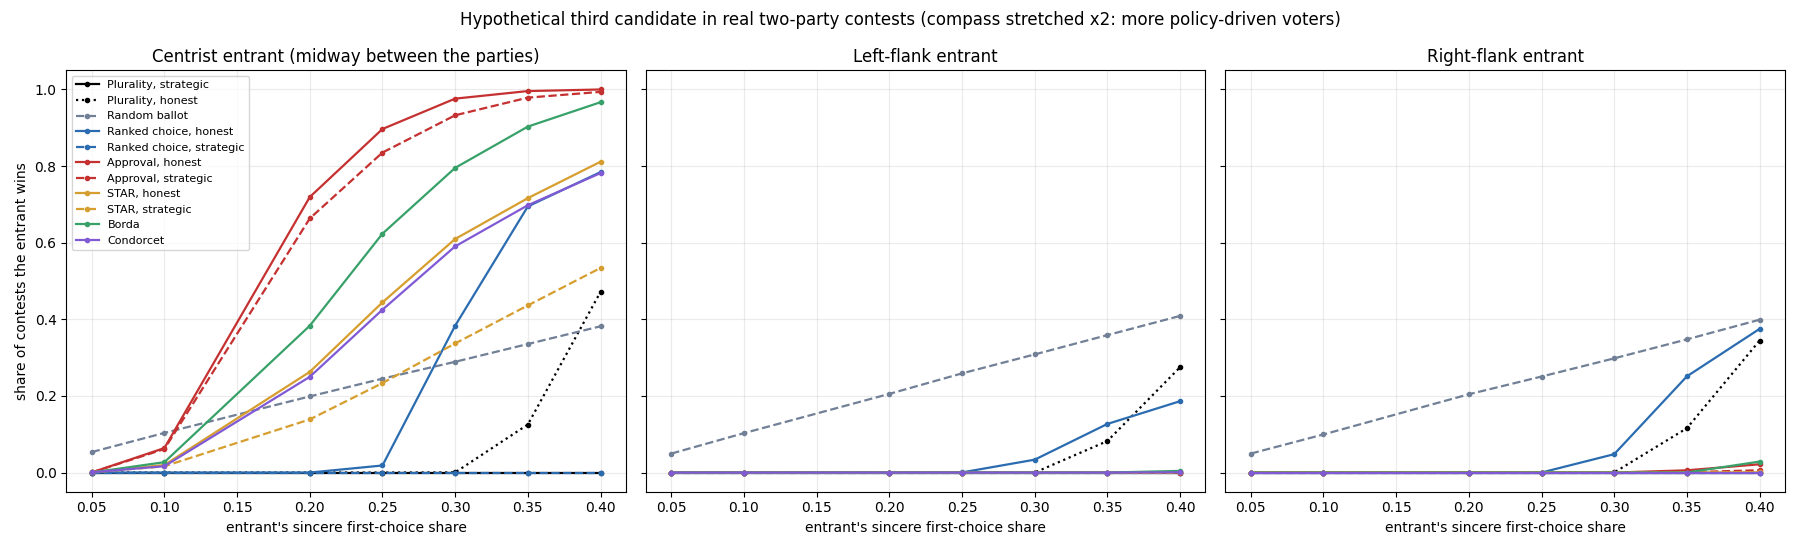
\includegraphics[width=\textwidth]{scenarios/entrant_wins_stretch2.png}
\caption{Entrant win rate by method on the stretched compass. Ranked choice excludes a centrist that approval, STAR and Condorcet elect, and elects flank candidates that they do not.}
\end{figure}

On the fitted compass the rules rarely disagree, because taste shocks are large relative to policy distances: a candidate with few first choices is also few voters' second choice. On the stretched compass ranked choice and approval diverge sharply (centre squeeze), and approval elects the centrist more often than head-to-head majorities would.

\paragraph{Pragmatic versus honest ranked choice.} In flank scenarios, ranking a major-party candidate first raises compass expression: fitted left flank at $40\%$, $-3.729$ (honest) to $-3.594$ (pragmatic); fitted right flank at $35\%$, $-3.660$ to $-3.594$; stretched right flank at $35\%$, $-3.699$ to $-3.594$. The corresponding honest-to-pragmatic changes for approval and STAR are $0$--$0.04$. Expression differences are small throughout (under $4\%$) because the fitted parties are close together relative to the voters.

\paragraph{Where approval is fragile.} On the real contests at $\rho=0$, the unweighted approval rule changes the winner in about $105$ more contests than sampling noise explains; pragmatic approval, ranked choice and STAR do not. In centrist scenarios all three rules are moved by pragmatic voting (fitted, centrist at $40\%$: entrant win rate $0.82\to0$ for ranked choice, $0.89\to0.55$ for approval, $0.82\to0.29$ for STAR).

\FloatBarrier
\subsection{Random ballot as a benchmark}
Averaged over 23 House elections at $\rho=0$, every deterministic rule is $19.5$--$19.9$ seats away from random ballot's expected party split, with Gallagher index $3.8$--$3.9$ against $0.3$ for random ballot. The spread among deterministic rules ($0.4$ seats) is negligible beside their distance from random ballot. Random ballot elects the head-to-head winner in $64\%$ of multi-candidate contests, against $96$--$100\%$ for the deterministic rules. Expected third-party House seats per election under random ballot are $9.6$, $11.1$, $15.5$, $26.6$ and $50.1$ for $\rho=0, 0.2, 0.5, 0.75, 0.9$.

\section{Measurement 2: suppression by year from one-major contests}
\label{sec:suppression}

\FloatBarrier
\subsection{Estimator}
In contests where only one major party ran there is no spoiler risk and the third candidate is the only alternative, so both strategic desertion and the ``not a serious contender'' discount are switched off. Using valences calibrated with $\rho=0$, define for each third-party candidate $j$ in contest $r$ the relative appeal $a_{rj}=v_{rj}-\max_{l\ \text{major}}v_{rl}$. We estimate
\begin{equation}
a_{rj} = \alpha_{t(r)} + \gamma_{g(j)} + \eta_{o(r)} - \Delta_{t(r)}\,\mathrm{two}_r + \kappa\,\mathrm{two}_r\,\mathrm{margin}_r + e_{rj},
\end{equation}
where $\mathrm{two}_r$ indicates that both a Democrat and a Republican ran, $g$ is the party group and $o$ the office. $\Delta_t$ is the log-odds gap in year $t$ and the suppression rate at a dead heat is $\rho_t = 1-e^{-\Delta_t}$. Yearly gaps are shrunk toward the precision-weighted pooled value $\bar\Delta$ by empirical Bayes,
\begin{equation}
\tilde\Delta_t = \bar\Delta + \frac{\hat\tau^2}{\hat\tau^2+\mathrm{se}_t^2}\,(\hat\Delta_t-\bar\Delta), \qquad \hat\tau^2=\max\!\big(0,\operatorname{Var}(\hat\Delta_t)-\overline{\mathrm{se}_t^2}\big).
\end{equation}
The sample is $7{,}313$ third-party candidates, $766$ of them in one-major contests.

\FloatBarrier
\subsection{Estimates}
Third-party candidates average $2.5\%$ when both majors run and $11.0\%$ when one does. The pooled gap is $\bar\Delta=1.66$ ($\rho=0.81$) with between-year s.d.\ $0.39$. The closeness coefficient is $\hat\kappa=-0.04\pm0.06$, indistinguishable from zero, and is not used. Even in one-major contests the mean relative appeal is $-1.50$ (Libertarian $-1.13$, Green $-1.41$, other $-1.73$): a residual gap that mixes candidate quality with perceived seriousness and is not removed below.

\begin{table}[H]\centering\small
\caption{Suppression by election year. Shares are mean third-party candidate shares; $\rho_t$ is the rate applied in the simulation.}
\begin{tabular}{rrrrrrrrr}
\toprule
Year & \multicolumn{2}{c}{Candidates} & \multicolumn{2}{c}{Mean share (\%)} & $\hat\Delta_t$ & s.e. & $\tilde\Delta_t$ & $\rho_t$ \\
 & one major & two majors & two majors & one major & & & & \\
\midrule
1976 & 28 & 227 & 2.3 & 9.8 & 1.36 & 0.19 & 1.42 & 0.76 \\
1978 & 24 & 156 & 3.2 & 8.1 & 1.33 & 0.21 & 1.40 & 0.75 \\
1980 & 24 & 233 & 2.7 & 6.2 & 0.93 & 0.20 & 1.09 & 0.66 \\
1982 & 39 & 240 & 1.7 & 6.1 & 1.29 & 0.16 & 1.35 & 0.74 \\
1984 & 19 & 140 & 1.7 & 6.7 & 1.42 & 0.23 & 1.48 & 0.77 \\
1986 & 30 & 125 & 2.0 & 5.3 & 0.84 & 0.19 & 1.01 & 0.63 \\
1988 & 26 & 164 & 1.9 & 8.0 & 1.69 & 0.20 & 1.68 & 0.81 \\
1990 & 31 & 145 & 3.8 & 12.4 & 1.07 & 0.19 & 1.18 & 0.69 \\
1992 & 24 & 427 & 3.2 & 10.3 & 1.19 & 0.20 & 1.28 & 0.72 \\
1994 & 21 & 262 & 2.7 & 10.7 & 1.29 & 0.22 & 1.37 & 0.75 \\
1996 & 5 & 490 & 2.2 & 7.0 & 2.12 & 0.43 & 1.87 & 0.85 \\
1998 & 70 & 356 & 1.9 & 11.7 & 2.09 & 0.13 & 2.05 & 0.87 \\
2000 & 63 & 500 & 2.2 & 10.3 & 2.23 & 0.13 & 2.18 & 0.89 \\
2002 & 66 & 336 & 2.2 & 11.0 & 1.98 & 0.13 & 1.95 & 0.86 \\
2004 & 37 & 306 & 2.1 & 11.4 & 2.05 & 0.17 & 1.99 & 0.86 \\
2006 & 33 & 264 & 2.4 & 15.3 & 1.87 & 0.18 & 1.83 & 0.84 \\
2008 & 40 & 296 & 2.8 & 11.7 & 1.25 & 0.16 & 1.31 & 0.73 \\
2010 & 21 & 453 & 2.7 & 14.4 & 1.94 & 0.21 & 1.87 & 0.85 \\
2012 & 39 & 326 & 2.6 & 14.6 & 1.99 & 0.16 & 1.94 & 0.86 \\
2014 & 52 & 277 & 2.7 & 13.3 & 1.69 & 0.14 & 1.69 & 0.81 \\
2016 & 33 & 298 & 3.1 & 13.6 & 1.75 & 0.18 & 1.74 & 0.82 \\
2018 & 31 & 261 & 2.3 & 11.9 & 1.30 & 0.18 & 1.36 & 0.74 \\
2020 & 10 & 265 & 2.1 & 18.4 & 2.39 & 0.31 & 2.12 & 0.88 \\

\bottomrule
\end{tabular}
\end{table}

\begin{figure}[!htbp]\centering
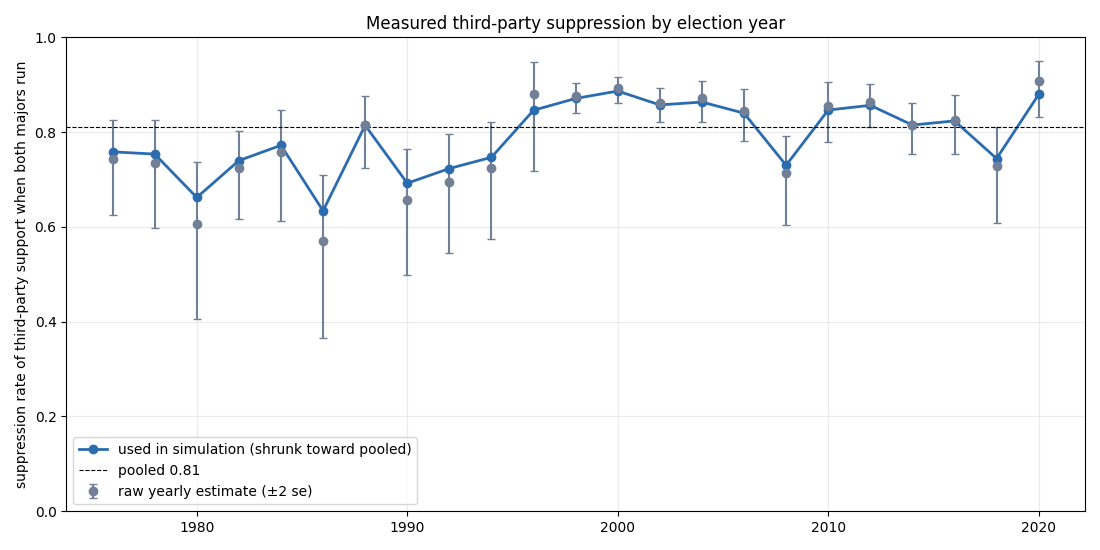
\includegraphics[width=0.8\textwidth]{desertion/suppression_by_year.png}
\caption{Measured suppression of third-party support by election year.}
\end{figure}

\FloatBarrier
\subsection{Suppression-adjusted baseline}
Each two-major contest receives its year's $\rho_t$ (capped as in Section~\ref{sec:strategy}; the cap binds in $518$ of $4{,}626$ adjusted contests). Valences are re-solved so that strategic plurality reproduces the real shares (largest error $6\times10^{-4}$). The implied sincere third-party first-choice share rises from $2.3\%$ to $8.0\%$. Agents then vote sincerely under every rule, 200 runs of $1{,}000$ agents.

\begin{table}[H]\centering
\caption{Suppression-adjusted baseline: third-party winners among $10{,}774$ contests (real: 19) and mean third-party seats per election.}
\begin{tabular}{lrrr}
\toprule
Method & Winners & House seats (real 0.5) & Senate chamber (real 1.0) \\
\midrule
Plurality, sincere & 110 & 3.8 & 2.3 \\
Ranked choice & 124 & 4.4 & 2.4 \\
Approval & 127 & 4.5 & 2.4 \\
STAR & 130 & 4.6 & 2.5 \\
Condorcet & 130 & 4.6 & 2.5 \\
Borda & 134 & 4.8 & 2.5 \\
Random ballot & 867 & 33.7 & 10.9 \\
\bottomrule
\end{tabular}
\end{table}

\begin{table}[H]\centering\small
\caption{Suppression-adjusted baseline: mean third-party House seats by year and method.}
\begin{tabular}{rrrrrrrrr}
\toprule
Year & Real & Plurality & RCV & Approval & STAR & Condorcet & Borda & Random \\
\midrule
1976 & 0 & 5.4 & 4.9 & 4.9 & 4.8 & 4.8 & 4.8 & 20.3 \\
1978 & 0 & 2.5 & 2.2 & 1.9 & 1.9 & 1.9 & 2.1 & 15.4 \\
1980 & 1 & 0.7 & 2.6 & 2.7 & 2.7 & 2.6 & 2.7 & 16.4 \\
1982 & 0 & 0.0 & 0.0 & 0.0 & 0.0 & 0.0 & 0.0 & 16.1 \\
1984 & 0 & 1.0 & 1.0 & 1.0 & 1.0 & 1.0 & 1.0 & 10.6 \\
1986 & 0 & 0.0 & 0.0 & 0.0 & 0.0 & 0.0 & 0.0 & 7.2 \\
1988 & 0 & 0.1 & 0.2 & 0.1 & 0.1 & 0.2 & 0.1 & 14.3 \\
1990 & 1 & 2.0 & 2.0 & 2.0 & 2.0 & 2.0 & 2.0 & 18.3 \\
1992 & 1 & 3.0 & 2.8 & 2.7 & 2.7 & 2.7 & 2.8 & 42.4 \\
1994 & 1 & 6.8 & 5.7 & 5.6 & 5.5 & 5.5 & 4.8 & 25.2 \\
1996 & 2 & 6.2 & 6.6 & 7.0 & 7.1 & 7.1 & 7.3 & 55.9 \\
1998 & 1 & 3.8 & 4.4 & 4.6 & 4.7 & 4.7 & 5.3 & 48.9 \\
2000 & 2 & 9.1 & 11.4 & 11.2 & 11.3 & 11.3 & 12.1 & 74.4 \\
2002 & 1 & 1.8 & 1.3 & 1.4 & 1.2 & 1.2 & 1.4 & 50.5 \\
2004 & 1 & 2.1 & 2.1 & 2.1 & 2.1 & 2.1 & 2.1 & 39.6 \\
2006 & 0 & 2.1 & 2.2 & 2.1 & 2.2 & 2.2 & 2.2 & 33.0 \\
2008 & 0 & 3.8 & 3.8 & 3.6 & 3.4 & 3.3 & 3.2 & 30.8 \\
2010 & 0 & 15.0 & 17.1 & 18.1 & 18.7 & 18.5 & 19.4 & 64.1 \\
2012 & 0 & 8.7 & 11.4 & 12.0 & 12.8 & 12.8 & 13.4 & 50.9 \\
2014 & 0 & 2.6 & 2.9 & 2.9 & 3.0 & 2.9 & 3.0 & 38.2 \\
2016 & 0 & 5.9 & 7.5 & 7.9 & 8.1 & 8.1 & 8.3 & 43.6 \\
2018 & 0 & 0.0 & 0.0 & 0.0 & 0.0 & 0.0 & 0.0 & 20.4 \\
2020 & 0 & 5.3 & 9.0 & 10.4 & 10.8 & 10.8 & 11.6 & 38.1 \\

\bottomrule
\end{tabular}
\end{table}

For House 2020 (real $222$ D, $212$ R) the Condorcet rule gives $221.6$ D, $201.6$ R, $4.0$ other, $6.9$ Libertarian; random ballot gives $210.7$, $185.2$, $16.1$, $22.0$. Run-to-run standard deviation is about $1.3$ House seats for the deterministic rules and $6.3$ for random ballot.

\begin{figure}[!htbp]\centering
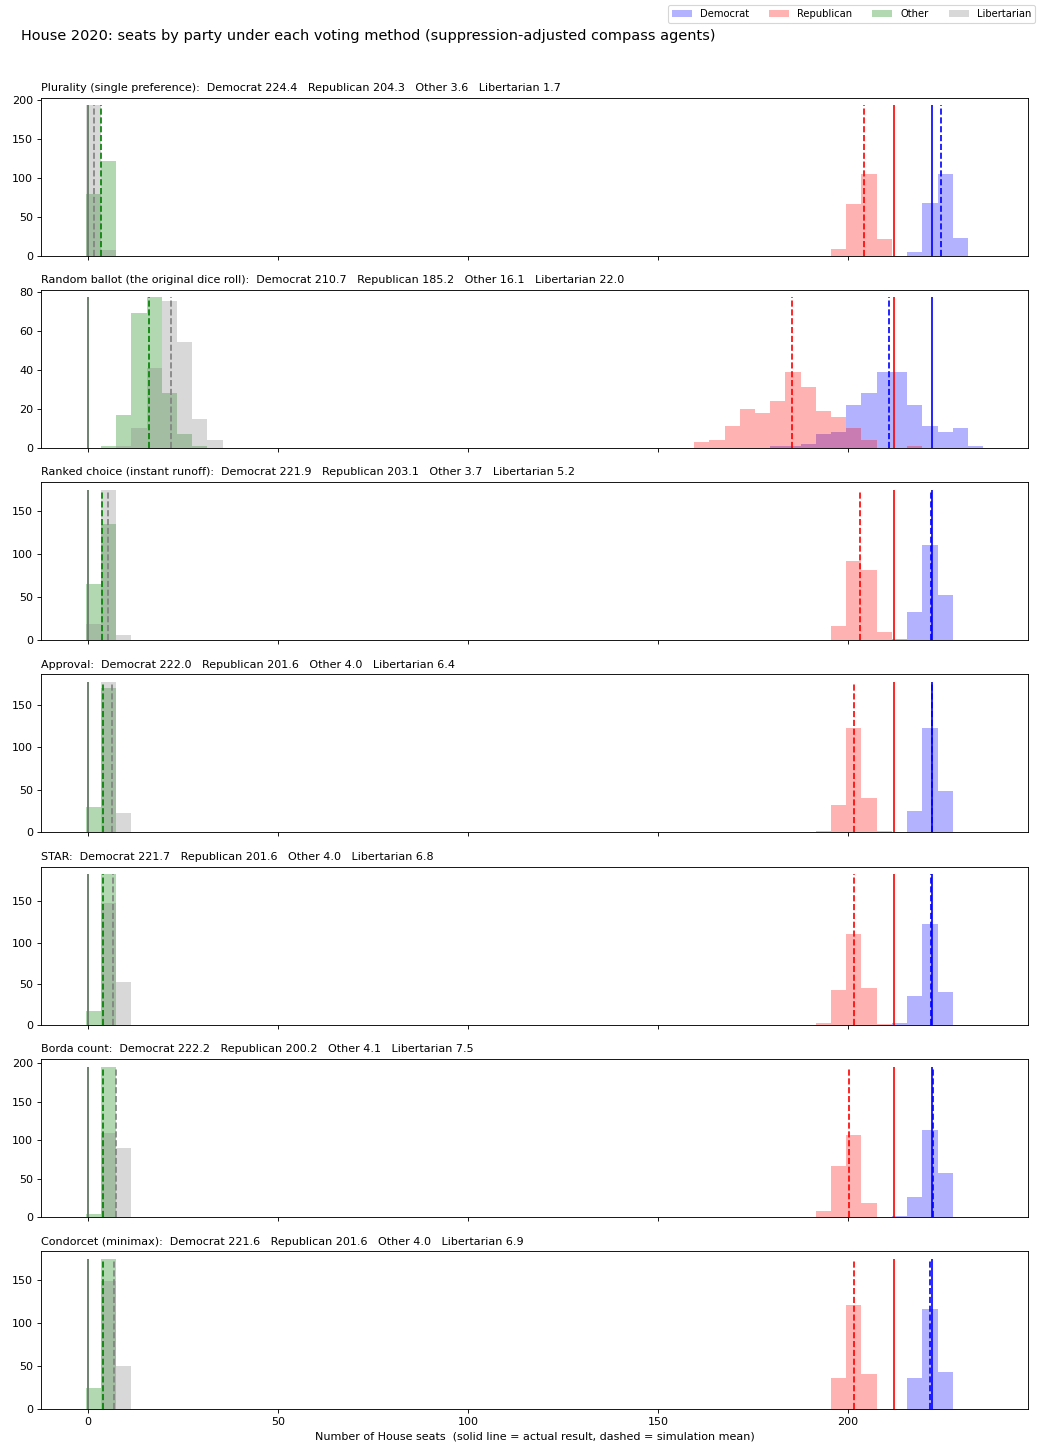
\includegraphics[height=0.70\textheight]{desertion/compare/house-methods-2020.png}
\caption{House 2020 under the suppression-adjusted baseline.}
\end{figure}

\FloatBarrier
\section{Limitations}
\begin{itemize}\itemsep2pt
\item \textbf{Point estimate.} The compass is a MAP fit. Reported intervals are predictive intervals for vote shares, not uncertainty over the compass.
\item \textbf{One identified axis.} The second dimension and the minor-party positions are weakly determined; results that depend on them (Borda, three-way races) are the least reliable.
\item \textbf{Suppression is bracketed, not pinned down.} The closeness gradient gives roughly zero once appeal is measured through the compass; the one-major comparison gives $0.64$--$0.89$ and is an upper estimate, because some of a third candidate's vote in a one-major contest comes from opposition partisans with no candidate, and the fitted parties are close together so that effect is absorbed into appeal. Candidates who choose to run in one-major contests may also differ.
\item \textbf{Uniform suppression within a year.} The adjusted baseline turns a real $7\%$ into roughly $46\%$ sincere (e.g.\ Illinois 13th district, 2012: $46.5/46.2/7.2$ becomes $28/26/46$). The implied claim, that third candidates above about $5\%$ would be sincere plurality favourites, is strong and testable against first-round counts where ranked choice is used.
\item \textbf{Fixed candidate field and limited strategies.} Entry, exit, and strategies such as burying or bullet voting are not modelled.
\item \textbf{Data.} Uncontested House races are excluded from fitting; there is no turnout model and no sub-national survey or demographic data; Senate ``real'' counts use general-election pluralities; a few House contests are missing in 1996 and 2006.
\item \textbf{Simulation size.} Scenario sweeps use 10--20 runs; differences of a few contests are noise.
\end{itemize}

\section{Tests that could falsify the main claims}
\begin{enumerate}\itemsep2pt
\item \textbf{Direct $\rho$.} In surveys that record candidate ratings and the vote (ANES, CES), the share of respondents who rate a third-party candidate highest but vote for a major party estimates $\rho$ directly.
\item \textbf{Adoption of ranked choice.} Third-party first-choice shares should rise by about $1/(1-\rho)$ where ranked choice replaces plurality. The fitted model predicts $3.7\%$ at $\rho=0.5$ and $8.0\%$ under the measured $\rho_t$, against $2.3\%$ observed.
\item \textbf{Second axis.} State-level issue surveys or roll-call scores for candidates would either stabilise the second dimension or show it is not there.
\item \textbf{Forward forecast.} A hold-out period not used in choosing the specification would give a clean out-of-sample test.
\end{enumerate}

\section*{Reproduction}
{\small
\begin{verbatim}
.venv/bin/python -m pytest tests -q
.venv/bin/python scripts/run_compass.py --offices PSH --split none --tag full_d2K4
.venv/bin/python scripts/run_methods.py
.venv/bin/python scripts/plot_methods.py
.venv/bin/python scripts/run_scenarios.py
.venv/bin/python scripts/plot_scenarios.py
.venv/bin/python scripts/run_desertion.py
\end{verbatim}}

\end{document}
